\chapter{Phideus: The Computational Probe}

\epigraph{\emph{The only way to test whether ratios organize information is to build something that tries to speak their language.}}{}



\section{The question and why it needed a machine}


The previous chapters carried the argument as far as conceptual elaboration alone could take it. If consonance can be more than an aesthetic label, if harmonic organization can act as a relational constraint and perhaps as a candidate regime of informational efficiency, then the theory has reached the point where it must submit itself to an instrument. Phideus is one of those instruments. It is the computational probe of HIT: not a machine built to prove the whole theory in a single stroke, but a program designed to ask under controlled conditions whether ratio-based descriptions alter cross-modal organization in measurable ways.

That is why machine learning enters the manuscript here, and why it must enter carefully. Phideus does not inherit benchmark culture as if the values of optimization were already the values of theory. Nor does it treat neural networks as an ontology. It treats them as scientific apparatus in the sense developed earlier in this manuscript: instruments that receive transduced traces of events, transform them under explicit architectural constraints, and return structured readouts that can be interpreted as evidence about the object the experiment has constructed. The right analogy is closer to a spectrometer than to a metaphysics of intelligence. A spectrometer does not create the wavelengths it displays, but neither does it reveal them without imposing an optical apparatus of its own. The same care applies here.

The concept that makes this inquiry specific is the descriptor. In Phideus, a descriptor is not a generic feature. It is a compact numerical summary of some hypothesized relational organization, computed from the signal and injected into the model as guidance. In the strongest cases, that organization is ratio-based or harmonic: local intervals, linear frequency ratios, harmonic amplitude structure, or recurrent proportional relations. In other cases, the descriptor is deliberately non-ratio and functions as a control, allowing the program to test whether any gain comes from harmonic structure itself or from richer guidance more generally. To give the model a descriptor is to tell it what kind of structure should matter while it learns a shared space. Different descriptors therefore do not merely add dimensions. They operationalize different hypotheses about what sort of relation might organize correspondence across modalities.

Operationally, Phideus begins with a paired dataset. Each example contains two modalities or domains that refer to the same event and are aligned at the relevant unit of analysis. In a first phase, those paired domains are piano audio and piano MIDI. In a second phase, they are speech and electroglottography. In a third phase, the target pair is stereo audio and Lissajous figures generated from the same parametric scene. In a fourth phase, the target pair is electrocardiography and photoplethysmography recorded from the same cardiac event. In every case, the dataset is organized into matched segments or windows so that the model sees two different inscriptions of the same temporal event rather than two unrelated signals. That pairing is the experimental base condition. 

From that paired data, Phideus builds a dual neural architecture. There is one encoder for each modality, because each signal has to be transduced into its own latent representation before comparison becomes possible. On top of those encoders sit projection heads that map both sides into a shared embedding space. The encoders vary by front: sometimes they are smaller Transformer or CNN-Transformer models trained from scratch for traceability; sometimes a later comparison regime introduces a stronger frozen backbone such as MERT or WavLM on one side of the pair. But the basic architecture remains a paired encoder system followed by learned projections into a common space.

The descriptor enters after that setup is in place. For each side of the pair, the program computes a compact numerical summary of some hypothesized relational structure directly from the raw data or from a lightly transformed version of it. That descriptor is then injected into the network through a chosen route, such as concatenation, cross-attention, attention bias, reverse cross-attention, or projection conditioning. The point is not simply to add more input. The point is to alter what kind of relation the model is allowed to privilege while learning correspondence between both domains. Only after that descriptor injection does the model produce the embeddings that are compared in the shared space.

Training then optimizes a representation-learning objective rather than a direct classifier. The two projected embeddings are trained under VICReg so that matched pairs become structurally compatible without collapsing to a degenerate solution. After training, the system is evaluated first as a retrieval machine: can one modality recover its correct partner in the other? Only then do the later analyses ask the harder questions about causality, geometry, and mechanism. In compressed form, the loop is:

$$
z_a = P_a(E_a(x_a), d_a), \qquad z_b = P_b(E_b(x_b), d_b)
$$

$$
\mathcal{L} = \mathcal{L}_{\mathrm{VICReg}}(z_a, z_b)
$$

Auxiliary probes, decoders, and downstream tests appear later as diagnostics of what the model has preserved or lost. The core experiment, however, is always this: build a descriptor, decide how it enters, and ask whether the shared geometry changes in a measurable and interpretable way.

That baseline-first rigor is crucial. Phideus does not begin by injecting descriptors and then celebrating whichever arm happens to score highest. It first trains an unguided model under the same paired data, encoder pair, projection heads, and loss. That baseline establishes the reference retrieval level and the reference geometry of the shared space under a fixed protocol. Only then are descriptor-guided arms introduced: the same paired data, evaluation protocol, and architecture are held fixed as tightly as possible while descriptor content and route of injection vary. Every positive claim in the chapter is therefore comparative. The question is never whether a guided model produces a large number in isolation, but whether it changes retrieval, alignment, information retention, or causal sensitivity relative to the baseline it was designed to challenge.

What would count as evidence under such a program? Retrieval alone is not enough. A result must be read across four dimensions at once. First comes retrieval: can the model find the correct cross-modal partner more reliably when guided than when left unguided? Second comes causal control: does any advantage come from the informational content of the descriptor rather than from the extra machinery built around it? Third comes geometry: does descriptor guidance reorganize the shared representational space, and if so in what way? Fourth comes mechanism: is the descriptor's effect invariant to route of injection, or does where and how it enters the model change the outcome? Phideus treats these four dimensions together as a convergent argument. A score without controls is ambiguous. A control without a reading of geometry is incomplete.


\section{Experimental design: four escalones, one logic}


The program was not designed as a single decisive experiment. It was staged. Here escalon names one experimental front or staged level of the same general program. Each escalon asks a harder version of the same question, and each one preserves enough comparability with the others that a result in one domain can discipline what may later be claimed in the next. The sequence moves from a domain with clean pairing and rich prior tooling toward domains where the shared event is harder to capture, the transduction changes more radically, or the ground truth becomes newly generable.

Escalon 1 begins in music, with paired piano audio and piano MIDI from MAESTRO v3.0.0. This is the most hospitable opening because the musical event is held constant while the inscription changes. Audio records the acoustic result. MIDI records the performed gesture as symbolic event structure. The audio side is encoded with MERT, a pretrained music model with roughly 330 million parameters; the MIDI side uses a smaller Transformer trained from scratch; both project into a shared 256-dimensional space under VICReg \parencite{li_2024,bardes_2022}. The question is clean: when two inscriptions of the same event are already aligned at the dataset level, does descriptor guidance produce a stronger and more structured shared space than an unguided baseline?

Escalon 2 keeps the cross-modal logic but removes the symbolic convenience. Here the pair is speech and electroglottography. A microphone captures the airborne pressure wave; an electroglottograph records impedance variation at the level of glottal contact. The two signals come from the same vocal event but from materially different physical interfaces. The dataset is French Lombard v1.1, with 38 speakers and 9,120 clips segmented into two-second windows with half-second overlap. The architectural logic remains dual-encoder and shared-space, but the regime is deliberately more traceable than Escalon 1: the first pass does not hide behind a foundation speech encoder, because the point of the initial front is to see whether descriptor signal becomes legible under a simple, auditable setup before stronger backbones are introduced.

Escalon 3 moves into a domain where ratio can be generated, heard, and seen with exact control: stereo audio paired with Lissajous figures. Here ground truth is deterministic. Each scene carries explicit parameters of ratio, phase, and amplitude, and those parameters organize both the XY trajectory and the visible topology of the figure. This front matters not only because it cleans up ambiguity, but because it creates a direct convergence with Beacon, the experiential and physiological branch of the program developed more fully in Chapter 12. Phideus approaches the same harmonic scene computationally; Beacon approaches it through physical excitation and experience. Escalon 3 is therefore the first point in the program where both probes can interrogate the same object from different sides.

Escalon 4 extends the question outside acoustics altogether. Electrocardiography and photoplethysmography record the same cardiac event through different physical principles, electrical and optical. If ratio-based organization proves informative there as well, then the hypothesis is no longer confined to musical or vocal phenomena.

The primary retrieval metric is defined conservatively. Let S be the minimum of recall at rank 10 in both cross-modal directions. The score is estimated over 500 queries drawn from structured candidate pools that include hard negatives, semi-hard negatives, and random distractors. Pool sizes reflect domain structure: 256 candidates in Escalon 1 and 128 in Escalon 2. A run is only as strong as its weaker direction. Uncertainty is estimated by grouped bootstrap on the relevant identity unit, musical piece in Escalon 1 and speaker in Escalon 2.

This staged design gives the whole chapter its structure. Escalon 1 asks whether the machinery works under relatively clean conditions. Escalon 2 asks whether cross-modal organization survives a genuine shift in sensor physics. Escalon 3 introduces deterministic parametric control and opens the first direct experimental convergence with Beacon. Escalon 4 carries the same logic into cardiovascular physiology. The sequence is therefore not just chronological. It is an experimental gradient from engineered clarity toward harder forms of physical and biological complexity.

\begin{table}[ht]
\centering
\caption{Experimental fronts of Phideus, ordered by difficulty and domain distance.}
\label{tab:phideus_fronts}
\footnotesize
\begin{tabularx}{\textwidth}{@{}lllXl@{}}
\toprule
Front & Modality A & Modality B & Dataset & Status \\
\midrule
Escalon~1 & Piano audio & Piano MIDI & MAESTRO v3.0.0 & Closed \\
Escalon~2 & Speech & EGG & French Lombard v1.1 & Closed (null) \\
Escalon~3 & Audio XY & Lissajous figure & Synthetic + Analog & In progress \\
Escalon~4 & ECG & PPG & BIDMC / MIMIC & Planned \\
\bottomrule
\end{tabularx}
\end{table}

\begin{figure}[ht]
\centering
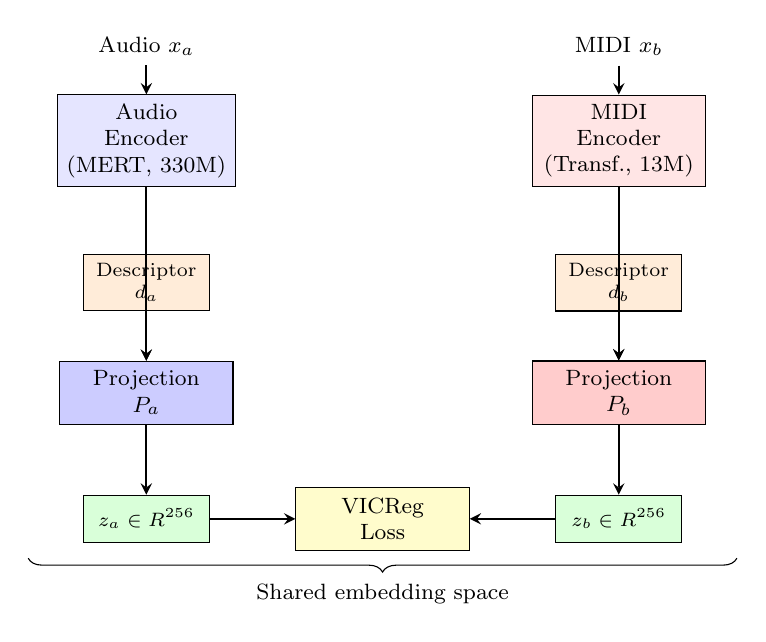
\begin{tikzpicture}[
    box/.style={rectangle, draw, minimum width=2.2cm, minimum height=0.8cm, align=center, font=\footnotesize},
    smallbox/.style={rectangle, draw, minimum width=1.6cm, minimum height=0.6cm, align=center, font=\scriptsize},
    arr/.style={->, thick},
    >=stealth
]
% Audio side
\node[box, fill=blue!10] (ea) at (-3, 0) {Audio\\Encoder\\(MERT, 330M)};
\node[smallbox, fill=orange!15] (da) at (-3, -1.8) {Descriptor\\$d_a$};
\node[box, fill=blue!20] (pa) at (-3, -3.2) {Projection\\$P_a$};
\node[smallbox, fill=green!15] (za) at (-3, -4.8) {$z_a \in \mathbb{R}^{256}$};

% MIDI side
\node[box, fill=red!10] (em) at (3, 0) {MIDI\\Encoder\\(Transf., 13M)};
\node[smallbox, fill=orange!15] (dm) at (3, -1.8) {Descriptor\\$d_b$};
\node[box, fill=red!20] (pm) at (3, -3.2) {Projection\\$P_b$};
\node[smallbox, fill=green!15] (zm) at (3, -4.8) {$z_b \in \mathbb{R}^{256}$};

% Input
\node[font=\footnotesize] (xa) at (-3, 1.2) {Audio $x_a$};
\node[font=\footnotesize] (xm) at (3, 1.2) {MIDI $x_b$};

% Loss
\node[box, fill=yellow!20] (loss) at (0, -4.8) {VICReg\\Loss};

% Arrows
\draw[arr] (xa) -- (ea);
\draw[arr] (ea) -- (pa);
\draw[arr] (da) -- (pa);
\draw[arr] (pa) -- (za);
\draw[arr] (xm) -- (em);
\draw[arr] (em) -- (pm);
\draw[arr] (dm) -- (pm);
\draw[arr] (pm) -- (zm);
\draw[arr] (za) -- (loss);
\draw[arr] (zm) -- (loss);

% Shared space bracket
\draw[decorate, decoration={brace, amplitude=5pt, mirror}] (-4.5, -5.3) -- (4.5, -5.3) node[midway, below=6pt, font=\footnotesize] {Shared embedding space};
\end{tikzpicture}
\caption{Architecture of the Phideus dual-encoder system. Each modality is encoded separately, guided by its descriptor, projected into a shared 256-dimensional space, and trained under VICReg loss. The descriptor injection point sits between encoder output and projection input.}
\label{fig:phideus_arch}
\end{figure}


\section{What counts as a descriptor in Phideus}


The word descriptor cannot do all the work by itself. Phideus needs three distinct terms. A descriptor is the informational structure injected into the model: what the model is being asked to attend to. A mechanism is the architectural route through which that structure enters: how it is injected. An arm is the concrete experimental combination of descriptor, mechanism, and training recipe. Keeping those terms separate is not pedantry. It is the only way to read the program without confusing content with route or route with full experimental condition.

For orientation, Table 11.2 below lists the descriptors themselves. Labels such as A4r or d4a4, which appear later in the chapter, do not name new descriptors but experimental arms built from those same descriptors under particular mechanisms.

That distinction clarifies several recurrent confusions at once. A4r is not a new descriptor; it is A4 under reverse cross-attention. Projection conditioning is not a descriptor; it is a mechanism for modulating the projection head. The canonical dual arm d4a4 is not a descriptor either; it is the experimental condition in which D4 guides the symbolic side and A4 guides the acoustic side. Once this vocabulary is fixed, the later results stop looking like a proliferation of unrelated labels and begin to read as controlled variations on a shared logic.

The descriptor-guided phase of Phideus was not the program's beginning. Earlier work explored denser and more literal representations of ratio structure: histograms of ratio distributions, sparse tokenizations inspired by acoustic fingerprinting, and exact matching schemes based on voting. Those experiments matter here only for one methodological lesson. Dense, temporally structured representations preserved enough organization to remain discriminative, while sparse matching and exact token logic tended to destroy the very cross-modal relation the program needed to learn. The move toward compact descriptors inside a learned embedding pipeline was therefore not arbitrary. It was the result of a prior elimination process.

Escalon 1 then made the descriptor problem operational without yet imposing a complete taxonomy over the whole program. It worked first with two pragmatic descriptors. D4 is a four-channel local interval descriptor on the MIDI side. For note \(i\), with MIDI pitch \(p_i\), it encodes the previous and next interval both in semitone and in octave-normalized log-ratio form:

$$
D4_i = \left[
\frac{p_i - p_{i-1}}{24},
\frac{p_{i+1} - p_i}{24},
\frac{\mathrm{clip}((p_i - p_{i-1})/12, -2, 2)}{2},
\frac{\mathrm{clip}((p_{i+1} - p_i)/12, -2, 2)}{2}
\right]
$$

A4 is the corresponding audio-side descriptor, computed from the temporal dynamics of log-magnitude in eight octave-like bands. If \(X_t(f)\) is the STFT magnitude at frame \(t\) and frequency bin \(f\), and \(B_b\) is octave band \(b\), then:

$$
\mu_b(t) = \frac{1}{|B_b|}\sum_{f \in B_b} \log(1 + |X_t(f)|),
\qquad
A4_t^{(b)} = \mu_b(t) - \mu_b(t-1)
$$

In implementation, these bandwise deltas are normalized and, when needed, interpolated to the target sequence length of the encoder side they guide. The important point for the present chapter is conceptual. D4 and A4 are descriptors. A4r is not a third descriptor but the arm in which A4 is injected through reverse cross-attention, and d4a4 is the dual arm in which D4 and A4 guide their respective modalities together. One descriptor is symbolic and explicitly local; the other is acoustic, broadband, and non-ratio in the strict sense. Together they were enough to establish the central closed result of the front, which Section 11.5 develops in full. But they did not yet settle the stronger question of natural harmony. A4 is spectrally rich without being a direct encoding of harmonic proportion, and D4 lives in a musically mediated interval space rather than in physically natural coordinates.

That is why the descriptor map of Phideus has to be read historically and experimentally rather than as a single universal family tree. Escalon 1 used D4 and A4 to prove that descriptor-guided cross-modal learning is a real and powerful mechanism. The retrospective music branch later reopened the question with A7, A9, and A10. Escalon 2 then introduced a new local taxonomy derived from the vocal oscillator itself. The point of the present section is not to flatten those moments into one scheme, but to make clear how they belong to the same program while preserving their different epistemic roles. Table 11.2 gives the compact map needed for the body of this chapter. The exhaustive inventory of descriptors, mechanism variants, and canonical arms belongs in Appendix C and in the companion methodological paper now in preparation, while the public Phideus repository carries the implementation-level detail.

\begin{table}[ht]
\centering
\caption{Inventory of descriptors across the Phideus program.}
\label{tab:descriptor_inventory}
\footnotesize
\begin{tabularx}{\textwidth}{@{}llclXX@{}}
\toprule
Front & Descriptor & Dim & Domain & What it encodes & HIT hypothesis \\
\midrule
Escalon~1 & D4 & 4 & MIDI & Local intervals & Symbolic relational structure \\
Escalon~1 & A4 & 8 & Audio & Spectral dynamics & Strong non-ratio control \\
Gate~9 & A7 & 12 & Audio & JI spectral ratios & Natural harmony retrospective \\
Gate~9 & A9 & 12 & Audio & JI spectral variant & Natural harmony retrospective \\
Gate~9/A10 & A10a--e & 6--32 & Audio & Recurrence-based ratios & Ontology-free relational encoding \\
\midrule
Escalon~2 & V4-lin & var & Speech & Linear $F_0$ ratios & Natural harmony in physical coords \\
Escalon~2 & V4-log & var & Speech & $\log_2 F_0$ ratios & Perceptual comparison \\
Escalon~2 & H-series & 12 & Speech & Harmonic amplitudes & Harmonic series structure \\
Escalon~2 & A4-16k & 8 & Speech & Spectral dynamics & Strong non-ratio control \\
\bottomrule
\end{tabularx}
\end{table}


\section{How descriptors enter the model: mechanism as variable}


If descriptors tell the model what kind of relation should matter, mechanisms determine how that guidance reaches the shared space. Phideus treats this not as implementation detail but as an experimental axis in its own right. A weak descriptor under one route may become productive under another. A strong descriptor may disappear if the route of injection is badly chosen.

Five mechanisms have structured the program so far. Concatenation appends descriptor values directly to encoder outputs:

$$
\tilde{h} = [h ; d]
$$

Cross-attention lets encoder features attend to descriptor tokens as an external source of guidance under the standard attention rule

$$
\mathrm{Attn}(Q,K,V) = \mathrm{softmax}\left(\frac{QK^{\top}}{\sqrt{d_k}}\right)V
$$

with \(Q=h\), \(K=d\), and \(V=d\). Attention bias perturbs self-attention more lightly, by modifying the attention logits from within the encoder without replacing the feature stream by descriptor tokens. Reverse cross-attention inverts the relation, using descriptor tokens as queries and encoder features as keys and values, so that \(Q=d\), \(K=h\), and \(V=h\). This proved especially useful in the retrospective music branch because it compresses long encoder sequences into a much smaller descriptor-guided interaction. Projection conditioning, inspired by FiLM, moves the intervention downstream and lets descriptor content modulate the mapping from encoder space into the shared space itself:

$$
h' = (1 + \gamma(d)) \odot h + \beta(d)
$$

This is the cleanest place in the program to see why descriptor and mechanism must not be collapsed. The same descriptor can behave very differently depending on whether it is concatenated, used as attention context, used as an attention query, or allowed to modulate the projection head late in the pipeline \parencite{vaswani_2017,perez_2018}.

The cleanest lesson of Escalon 1 is that route matters. Attention-based injection systematically outperforms simple concatenation, which means descriptor signal is not best understood as static side information pasted onto an embedding. It becomes productive when it is allowed to reorganize interaction among tokens. Projection conditioning adds a second lesson. Descriptor information can survive even when the intervention occurs at the end of the pipeline rather than at its beginning. The signal is therefore not tied to one privileged insertion point. It can work by reshaping token interaction early or by modulating the final projection late.

This distinction also stabilizes the reading of the chapter's own evidence. D4 and A4 answer the question of content. Concat, cross-attention, attention bias, reverse cross-attention, and projection conditioning answer the question of route. Arms such as d4a4, a4r, or d4-a4r belong to the level where both variables meet. Figure 11.2 schematizes the three most legible routes, while Appendix C and the methodological paper will carry the full implementation-level inventory. The later sections can then read results without collapsing these layers into one another.

\begin{figure}[ht]
\centering
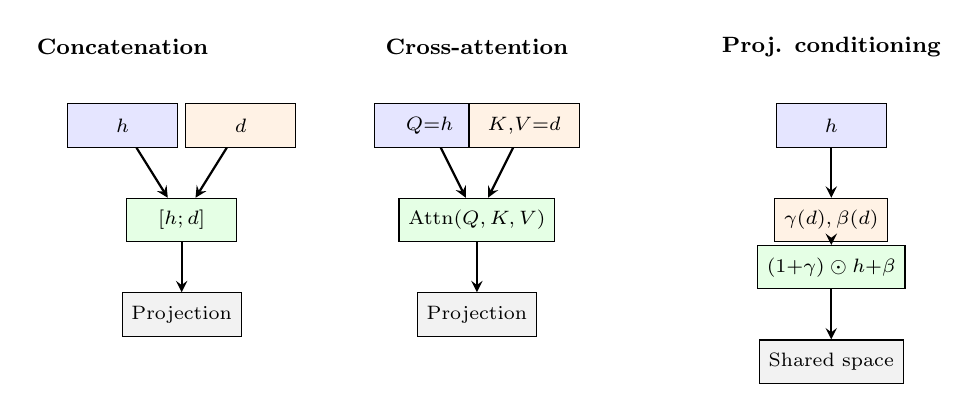
\begin{tikzpicture}[
    box/.style={rectangle, draw, minimum width=1.4cm, minimum height=0.55cm, align=center, font=\scriptsize},
    arr/.style={->, thick},
    >=stealth,
    every node/.style={font=\scriptsize}
]
% --- Concatenation ---
\node[font=\footnotesize\bfseries] at (-4.5, 2.2) {Concatenation};
\node[box, fill=blue!10] (c_h) at (-4.5, 1.2) {$h$};
\node[box, fill=orange!10] (c_d) at (-3.0, 1.2) {$d$};
\node[box, fill=green!10] (c_cat) at (-3.75, 0) {$[h ; d]$};
\node[box, fill=gray!10] (c_p) at (-3.75, -1.2) {Projection};
\draw[arr] (c_h) -- (c_cat);
\draw[arr] (c_d) -- (c_cat);
\draw[arr] (c_cat) -- (c_p);

% --- Cross-attention ---
\node[font=\footnotesize\bfseries] at (0, 2.2) {Cross-attention};
\node[box, fill=blue!10] (x_h) at (-0.6, 1.2) {$Q{=}h$};
\node[box, fill=orange!10] (x_d) at (0.6, 1.2) {$K{,}V{=}d$};
\node[box, fill=green!10] (x_att) at (0, 0) {Attn$(Q,K,V)$};
\node[box, fill=gray!10] (x_p) at (0, -1.2) {Projection};
\draw[arr] (x_h) -- (x_att);
\draw[arr] (x_d) -- (x_att);
\draw[arr] (x_att) -- (x_p);

% --- Projection conditioning ---
\node[font=\footnotesize\bfseries] at (4.5, 2.2) {Proj. conditioning};
\node[box, fill=blue!10] (f_h) at (4.5, 1.2) {$h$};
\node[box, fill=orange!10] (f_d) at (4.5, 0) {$\gamma(d), \beta(d)$};
\node[box, fill=green!10] (f_film) at (4.5, -0.6) {$(1{+}\gamma)\odot h{+}\beta$};
\node[box, fill=gray!10] (f_p) at (4.5, -1.8) {Shared space};
\draw[arr] (f_h) -- (f_d);
\draw[arr] (f_d) -- (f_film);
\draw[arr] (f_film) -- (f_p);
\end{tikzpicture}
\caption{Three descriptor injection mechanisms. \textbf{Left}: concatenation appends descriptor dimensions to encoder output. \textbf{Center}: cross-attention lets encoder features attend to descriptor tokens. \textbf{Right}: projection conditioning modulates the projection head via a learned affine transformation (FiLM).}
\label{fig:injection_mechanisms}
\end{figure}


\section{The central result: descriptor-guided cross-modal learning works}


The strongest closed result of Phideus remains the multi-seed validation of the canonical dual arm in Escalon 1. Across five independent seeds, d4a4 reaches a mean S of 84.1 percent with a standard deviation of 2.3 percentage points, while the unguided baseline D0 reaches 75.2 percent with the same standard deviation. The effect size is large, Cohen d = 4.50, and the distributions do not overlap: the weakest guided seed remains above the strongest unguided one. The result is not a fortunate run. It is a stable shift in the behavior of the system, and it must be read against the explicit pipeline just defined: descriptor content, route of injection, projection into shared space, and only then retrieval.

That retrieval advantage is supported by three causal lines of evidence. The first is inference-time ablation. When the A4 signal is zeroed at evaluation while keeping the trained weights fixed, performance collapses from 83.8 percent to 7.8 percent. The descriptor is not acting as decorative side information. The model depends on it. The second is parameter-matched degradation. Random, zeroed, or temporally shuffled substitutes fall back to the unguided band, leaving a causal gap of 9.4 percentage points between the real descriptor and the strongest degraded control. The advantage therefore comes from structured information rather than from added capacity alone. The third is pre-registration. Prediction matrices and admissible inference rules were written before the main readout, constraining interpretation before the relevant numbers were seen. That control does not make post-hoc reasoning impossible, but it sharply limits the most common forms of confirmation drift \parencite{pearl_2009}.

The evidence does not stop at retrieval. Cross-encoder alignment, measured by CKA, rises by roughly 82 percent in the guided condition, from 0.435 in D0 to as high as 0.794 in the best aligned arm \parencite{kornblith_2019}. At the same time, the descriptor-guided arms preserve roughly 29 percent more cross-modal information before the projection bottleneck. The descriptor is therefore not merely helping the model rank partners more effectively. It is altering the geometry through which both encoders are brought into relation.

Mechanistic evidence strengthens the same reading. Under projection conditioning, the best arm reaches 84.2 percent, the program's highest single-seed retrieval score. Even when only one side is conditioned late in the pipeline, the guided arm remains above the unguided control. Descriptor signal survives injection at the level of the projection head itself. This matters because it shows that the effect is not tied only to early token interaction. Guidance can remain operative all the way down to the final mapping into shared space.

The front also closes strongly at the level of discrimination difficulty. Descriptor-guided arms sustain hard-negative accuracy above 94 percent. These negatives come from the same musical piece at different temporal locations, so timbre, recording conditions, and style remain nearby while local identity changes. The model is not merely learning piece signature. It is learning temporal correspondence with fine resolution.

\begin{table}[ht]
\centering
\caption{Summary of convergent evidence, Escalon~1.}
\label{tab:escalon1_evidence}
\footnotesize
\begin{tabularx}{\textwidth}{@{}lllX@{}}
\toprule
Dimension & Test & Result & Interpretation \\
\midrule
Retrieval & Multi-seed replication & $84.1\% \pm 2.3$pp & Replicable advantage, $d = 4.50$ \\
Causal (ablation) & Inference-time zeroing & $83.8\% \to 7.8\%$ & Descriptor causally necessary \\
Causal (controls) & Parameter-matched degradation & $+9.4$pp gap & Information, not parameters \\
Geometric & CKA alignment & $+82\%$ & Representational reorganization \\
Information & Pre-projection retention & $+29\%$ & More cross-modal info preserved \\
Mechanistic & Projection conditioning & $84.2\%$ (record) & Signal survives deep in pipeline \\
Fine-grained & Hard negatives & $> 94\%$ & Temporal identity, not just piece \\
\bottomrule
\end{tabularx}
\end{table}

\begin{table}[ht]
\centering
\caption{Multi-seed replication of cross-modal retrieval, Escalon~1 ($n = 5$ seeds).}
\label{tab:escalon1_multiseed}
\footnotesize
\begin{tabular}{@{}lcccccc@{}}
\toprule
Arm & Mean $S$ & SD & Range & $\Delta$ vs D0 & Cohen $d$ & Sig. \\
\midrule
d4a4 & 84.1\% & 2.3pp & 82.0--86.4 & $+8.9$pp & 4.50 & $p < 0.001$ \\
d4-a4r & 81.2\% & 2.5pp & 78.4--83.4 & $+6.0$pp & 2.50 & $p < 0.01$ \\
a4r & 80.7\% & 1.9pp & 79.4--84.0 & $+5.5$pp & 2.63 & $p < 0.01$ \\
D0 & 75.2\% & 2.3pp & 71.8--77.4 & --- & --- & baseline \\
\bottomrule
\end{tabular}
\end{table}


\section{The second front: speech and electroglottography}


Escalon 2 poses a harder question than Escalon 1 because the modalities are no longer separated by notation versus acoustics. Speech is an airborne pressure wave. Electroglottography measures glottal contact through impedance. The event is shared, but the transduction is materially different from the start. Whatever cross-modal structure the model learns to use here has survived a genuine change in sensor physics.

That is why the unguided baseline matters so much. Under grouped bootstrap by speaker, D0 reaches 77.8 percent. On its own, that number already establishes something important: speech and electroglottographic traces share enough organization for a neural model to retrieve one from the other at a high level over structured candidate pools. Cross-modal structure in Phideus is therefore not confined to music, symbolic pairing, or aligned score metadata.

The first descriptor-guided pass over the vocal front was not framed as a failure hunt but as a mechanistic clarification. Twelve conditions were tested across descriptor families and routes of injection. None produced a defendable lift over D0 under the declared interpretive rules. That closes one easy reading and does something more valuable than a premature positive would have done: it shows that the front cannot be carried by weak wins under the current encoder regime. The existence claim is already secure at the level of the baseline. The open question is now more precise. Under what representational conditions does descriptor signal become legible in this harder domain?


\section{The discovery: representation organizes geometry}


The program's deepest finding is not exhausted by any single retrieval score. It is a structural discovery about what descriptor guidance does to representation.

The finding can be stated simply. Descriptor-guided models are not more linearly decodable than the unguided baseline. Ridge probes over the shared space return comparable or slightly weaker linear readout. And yet those same guided models show dramatically stronger cross-encoder alignment under CKA, along with higher information retention before the projection bottleneck. The descriptor does not simply add content that can be read out as one more feature. It reorganizes the shared geometry in which both modalities are brought into relation.

The descriptor does not enrich what the model knows. It reorganizes how the model relates what it already knows across modalities.

That distinction matters for the theory because it connects directly to the relational ontology developed earlier in the manuscript. If information is not exhausted by isolated substance but also lives in organized relation, then geometric reorganization is not a consolation prize below "real" performance. It is one of the most direct ways a system can show that a compact relational signal is constraining the field within which correspondence is learned. The effect disappears when descriptor content is degraded, which makes the reading stronger still. Ratio-based guidance is acting less like additive enrichment and more like geometric constraint.


\section{Phideus as constructive process}


Phideus is not merely observational. It is constructive. The program does not only ask whether ratio-based organization is present in signals. It builds models that attempt to learn under ratio-based guidance and then asks what changes in the resulting cross-modal space. That move matters because it turns a theoretical intuition into an engineering pressure test.

The constructive posture also imposes its own rigor. A descriptor may improve a model for reasons that do not validate the larger theory. It may regularize training, stabilize a bottleneck, or provide auxiliary structure without proving anything strong about harmony as such. The inverse can also happen: a theoretically important descriptor can fail because it was injected poorly, measured crudely, or tested under the wrong architectural comparison. Engineering utility and theoretical confirmation therefore cannot be treated as synonyms. Keeping them separate is not a weakness of the program. It is one of the conditions that makes the computational branch scientifically usable.

The next fronts extend that constructive logic without exhausting it. Escalon~3 will bring ratio into a domain where it is exactly specifiable, visible, and audible at once, creating the first experimental convergence with Beacon around Lissajous objects. Escalon~4 will ask whether the same general question can survive outside acoustics in cardiovascular physiology. Phideus can make harmonic hypotheses operational, but it cannot close the entire phenomenon from inside computation alone. The next chapter takes up the complementary task: what becomes visible when the same problem is probed through sustained acoustic fields, embodied response, and acoustic-physiological experience.


\section{Experimental implications of the activation conjecture}

Chapter~10 matters here because it sharpens what a computational probe should ask. If storage and retrieval are formally distinct, then a learned latent space should not be tested only with the same relational logic that helped stabilize it. It should also be tested with queries that challenge the space without simply collapsing into arbitrary noise. In practical terms, that means Phideus can compare integer-ratio probes, consonant neighborhoods, and $\varphi$-offset or noble-number perturbations as different ways of asking what a learned manifold preserves, when it locks, and when it becomes newly readable.

The point is not to turn Phideus into a golden-ratio machine. The point is to give the computational branch a sharper family of contrasts. A ratio-guided descriptor may help organize storage-like regularity in the latent space. A $\varphi$-offset query may help reveal whether that organization can be activated, traversed, or read without being overwritten by the same commensurate logic that produced the lock in the first place. That distinction creates a more exact experimental vocabulary for the fronts already named in this chapter, especially where the object is explicitly geometric or phase-bearing.
